\chapter{模型评估}\label{chap:experiments}

\section{引言}\label{sec:map-to-real}
本章将在MNIST\citep{lecun1989backpropagation}和FashionMNIST\citep{xiao2017/online}数据集上评估模型。MNIST是深度学习广泛使用的评价模型的基础数据集,它包含60000个训练样本,10000个测试样本,每个样本均为$28\times 28$的灰度手写数字图片。FashionMNIST具有和MNIST相同的数据结构,训练样本数量和测试样本数量均与MNIST相同,每个样本也都是$28\times 28$灰度图片,也具有10个类别。然而相较于MNIST,FashionMNIST的图片构成更为复杂,因此对模型具有更大的挑战。

在所有实验中,本文主要考察两个指标:分类准确率和图片生成质量。对于分类准确率,计算模型预测值并不像一般分类器那样直接。隐变量虽然可以学习到数据类别的特征,但是其取值并不一定和真实标签正确对应(例如$c=1$对应生成真实标签为$\omega_2$的数据)。因此不能直接使用隐变量的取值作为模型的预测值,必须将隐变量的取值与真实标签之间做一个映射。

对于这个问题,本文采取与\citet{springenberg2015unsupervised}类似的做法。首先在测试集上选取$t$个测试样本$\Set{X}_t = \{\mathbf{x}_i, y_i\}_{i=1}^t$,计算模型在这批数据上的预测概率矩阵
\[
  \mathbf{P} = 
\begin{bmatrix}
  p_{11} & p_{12} & \cdots & p_{1k} \\
  p_{21} & p_{22} & \cdots & p_{2k} \\
  \vdots & \vdots & \ddots & \vdots \\
  p_{t1} & p_{t2} & \cdots & p_{tk}
\end{bmatrix},
\]
其中$p_{ij} = \Pr(y=\omega_j | \mathbf{x}_i)$表示给定输入样本$\mathbf{x}_i$时,模型预测$y = \omega_j$的概率。然后对每一行选取最大概率的索引作为模型在这批样本上的预测值
\[
  \mathbf{P}^{\star} = (\ell_1, \ell_2, \cdots, \ell_t)^T, \quad \ell_i = \argmax_j p_{ij}.
\]
显然$\ell_i, ~y_i \in \Omega = \{\omega_1, \omega_2, \cdots, \omega_K\}$。定义映射$f: \Omega \to \Omega$,
\[
  f(\ell) = \argmax_y \left( 
    \sum_{\mathbf{x}: \ell(\mathbf{x}) = \ell} \mathbf{1}\Big(y(\mathbf{x}), y\Big) 
  \right),
\]
其中$\ell(\cdot)$表示给定输入下模型预测的虚假标签,$y(\cdot)$表示给定输入的真实标签,$\mathbf{1}(a, b) = 1$当且仅当$a = b$, 否则为零。此时,给定模型预测的虚假标签$\ell$,映射$f$都可以将它映射为真实标签$f(\ell)$。这就完成了虚假标签到真实标签的转换\footnote{在实际应用中,可能会出现某一行的最大值不唯一的情况,此时选择第一个最大值索引作为输出。值得注意的是,这种情况在实验中并不多见。}。简单来说,模型为每一个数据$\mathbf{x}_i$输出对应的概率向量$p(y|\mathbf{x}_i)$,从而分配虚假标签$\ell_i$(概率向量中最大概率对应的索引),然后将预测值和真实标签对比:将虚假标签落入最多的真实标签的取值作为该虚假标签的取值。比如在所有10个被分类为虚假标签$\ell_1$的样本中,有9个真实标签为$\omega_3$,则将虚假标签$\ell_1$映射到真实类别$\omega_3$。

对于图片生成质量,本文采用Fréchet Inception Distance (FID)\citep{heusel2017gans}来进行衡量\footnote{FID一般用于彩色图片,而MNIST数据集是单通道的灰度图片,本文的做法是把单通道复制3份,形成一张RGB彩色图片然后再计算其FID值。}。相较于Inception Score\citep{salimans2016improved}只考虑生成数据,FID还利用了真实数据,因此更能反映生成数据和真实数据的差异。FID越小代表生成的图片和真实图片越接近,生成质量越好。

\begin{figure}[htb]
  \centering
  \begin{subfigure}[b]{\trif\textwidth}
    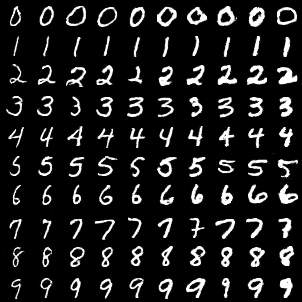
\includegraphics[width=\textwidth]{Img/icg-width.png}
    \caption{$c_2$调控生成数字的粗细}
    \label{ffig:m-icg-witdth}
  \end{subfigure} 
  \begin{subfigure}[b]{\trif\textwidth}
    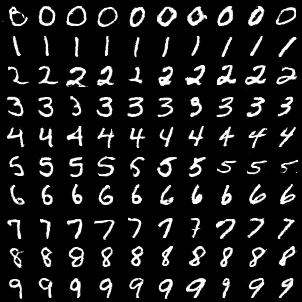
\includegraphics[width=\textwidth]{Img/icg-rotation.png}
    \caption{$c_3$调控生成数字的角度}
    \label{ffig:m-icg-rotation}
  \end{subfigure} 
  \begin{subfigure}[b]{\trif\textwidth}
    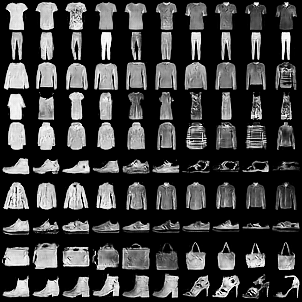
\includegraphics[width=\textwidth]{Img/icg-light.png}
    \caption{$c_2$调控生成图片的亮度}
    \label{ffig:fa-icg-light}
  \end{subfigure} 
  \bicaption[隐变量对生成图片的调控]
  {隐变量对生成图片的调控。图中每一行对应类别隐变量的一个取值,每一列对应其他某个隐变量(固定剩余隐变量)的连续变化。}
  {The control of latent variables on the generated pictures. Each row in the figure corresponds to a value of the category latent code, and each column corresponds to variants of a continuous code with other codes fiexd.}
  \label{fig:latent-varies}
\end{figure}

\section{实现细节}
在实践中,模型中的所有模块(生成器、判别器、辅助网络等)均被实现为深度神经网络。实验代码托管于Github\footnote{代码地址:\url{https://github.com/guyueshui/InfoCatGAN}}。

\subsection{C-InfoGAN}
对于C-InfoGAN模型,实验的设定和InfoGAN大致相同。辅助网络$Q$和判别器$D$共享前部网络结构,$Q$在判别器的尾部(通常是倒数第二层)分离出一个全连接网络,输出后验概率的估计$Q(\bd{c}|\bd{x})$。因此,C-InfoGAN带来的计算复杂度增加较小。对于离散隐变量$c_i$,在输出之前施加一个softmax激活层,得到的输出代表$Q(c_i|\bd{x})$。对于连续隐变量$c_j$,我们假设其先验分布为高斯分布,然后利用$Q$网络输出它的均值和方差,放到高斯分布中去拟合,计算差值。
由于GAN在训练时容易坍塌,DCGAN\citep{radford2015unsupervised}提出了一种训练稳定的生成对抗网络结构,所以实验中采用的网络结构对此有很多参考。若无特别说明,实验中超参数$\lambda_1$(参见\eqref{eq:cinfogan-obj}式)沿用InfoGAN的设定,对于离散隐变量设置为1,对于连续隐变量设置为0.1;$\lambda_2$设置为1,在半监督情况下,引入的交叉熵系数$\lambda_3$(参见\eqref{eq:ss-cinfogan-obj}式)设为1。

\begin{table}[htbp]
  \renewcommand\arraystretch{0.7} % set row height
  \centering
  \bicaption{C-InfoGAN在MNIST上的网络结构}
  {Architectures of C-InfoGAN used for MNSIT dataset}
  \begin{tabular}{l|l}
    \toprule
    \textbf{生成器$G$}                        & \textbf{判别器$D$/辅助网络$Q$} \\ \midrule
    Input $\in \reals^{74}$                   & Input $28\times 28$ Gray image \\ \hline
    FC. 1024 ReLU. bn                         & $4\times 4$ conv. 64 lReLU. bn  \\ \hline
    FC. $7\times7\times128$ ReLU. bn          & $4\times 4$ conv. 128 lReLU. bn \\ \hline
    $4\times 4$ upconv. 64 ReLU. stride 2. bn & FC. 1024 lReLU. bn \\ \hline
    ~                                         & FC. 1 sigmoid. output for $D$, \\
    $4\times 4$ upconv. 1 Tanh. stride 2      & FC. 128-bn-lReLU-FC. output for $Q$ \\
    \bottomrule
  \end{tabular}
  \label{tab:m-cig-netarch}
\end{table}
\begin{table}[htbp]
  \renewcommand\arraystretch{0.7} % set row height
  \centering
  \bicaption{C-InfoGAN在FashionMNIST上的网络结构}
  {Architectures of C-InfoGAN used for FashionMNSIT dataset}
  \label{tab:fm-cig-netarch}
  \begin{tabular}{l|l}
    \toprule
    \textbf{生成器$G$}                        & \textbf{判别器$D$/辅助网络$Q$} \\ \midrule
    Input $\in \reals^{74}$                   & Input $28\times 28$ Gray image \\ \hline
    $1\times 1$ upconv. 1024 ReLU. bn         & $4\times 4$ conv. 64 lReLU. stride 2  \\ \hline
    $7\times 7$ upconv. 128 ReLU. bn          & $4\times 4$ conv. 128 lReLU. stride 2. bn \\ \hline
    $4\times 4$ upconv. 64 ReLU. stride 2. bn & $7\times 7$ conv. 1024 lReLU. bn \\ \hline
    ~                                         & $1\times 1$ conv. 1 sigmoid. output for $D$, \\
    $4\times 4$ upconv. 1 sigmoid. stride 2   & conv-128-bn-lReLU-conv. output for $Q$ \\
    \bottomrule
  \end{tabular}
\end{table}

表~\ref{tab:m-cig-netarch}给出了C-InfoGAN在MNIST上的网络结构,其中各缩写的意义为:FC表示全连接层;conv表示卷积层;upconv表示反卷积层;bn表示batch normalization, lReLU表示leaky rate为0.1的LeakyReLU激活函数。
如前所述,判别器$D$和辅助网络$Q$共享前部网络结构。在MNIST数据集上,噪声空间的构成为一个10维离散隐变量,两个连续隐变量和62维高斯噪声,最终得到的噪声维度为74。对于FashionMNIST,隐变量和噪声维度的设定同MNIST。实验中发现采用基于DCGAN的网络结构能够达到更好的效果,具体结构见表~\ref{tab:fm-cig-netarch}。


\subsection{InfoCatGAN}
通常情况下GAN的训练很不稳定。首先,如果判别器学习得太快,则\eqref{eq:gan-obj}式可能变得不稳定(此时生成器的损失函数梯度消失)。
%其次,生成器可能无法生成某一种数据模式,或者可能在不同模式之间疯狂切换。所以我们采取了两项措施来稳定训练。首先,在生成器和判别器中使用batch normalization。这有助于限制activation map,在实践中我们发现它可以防止生成器的模式切换以及在少数标签情况下提高判别器的泛化能力。值得一提的是,
其次,生成器可能无法生成某种特定的模式;或者是只能生成某种特定的模式而无法生成其它模式。对于这个问题,可以在实验中引入batch normalization,这样可以限制激活输出中的每个值的大小,并且实践证明加入batch normalization可以让生成器生成的图像更稳定。表~\ref{tab:m-icg-netarch}给出了InfoCatGAN的网络结构。在MNIST数据集上,InfoCatGAN的噪声空间的构成和C-InfoGAN类似,不同的是此处没有连续隐变量,即包含一个10维离散隐变量和一个128维高斯噪声,最终得到的噪声维度为138,其中perforated up-sampling表示\citet{dosovitskiy2015learning,osendorfer2014image}提出的反卷积方法。对FashionMNIST也使用同样的配置。若无特殊说明,实验中超参数(参见\eqref{eq:infocatgan}式)$\lambda_1 = 0.9$,半监督条件下(参见\eqref{eq:ss-infocatgan-obj}式)$\lambda_2 = 1$。

\begin{table}[h]
  \renewcommand\arraystretch{0.7} % set row height
  \centering
  \bicaption{InfoCatGAN在MNIST上的网络结构}
  {Architectures of InfoCatGAN used for MNSIT dataset}
  \begin{tabular}{l|l}
    \toprule
    \textbf{生成器$G$}                    & \textbf{判别器$D$} \\
    \midrule
    Input $\in \reals^{138}$              & Input $28\times 28$ Gray image \\ \hline
    FC. $8\times8\times96$ lReLU. bn      & $5\times 5$ conv. 32 lReLU. bn \\ \hline
    $2\times2$ perforated up-sampling    & $3\times 3$ max-pool. stride 2. bn \\ \hline
    $5\times 5$ conv. 64 ReLU. bn        & $3\times 3$ conv. 64 lReLU. bn \\ 
    ~                                    & $3\times 3$ conv. 64 lReLU. bn \\ \hline
    $2\times 2$ perforated up-sampling   & $3\times 3$ max-pool. stride 2. bn \\ \hline
    $5\times 5$ conv. 64 lReLU. bn		  & $3\times 3$ conv. 128 lReLU. bn \\ 
    ~                        			  & $1\times 1$ conv. 10 lReLU. bn \\
    $5\times 5$ conv. 1 sigmoid		     & $5\times 5$ avg-pool. bn, 10-way softmax \\
    \bottomrule
  \end{tabular}
  \label{tab:m-icg-netarch}
\end{table}

\section{实验结果}\label{sec:results}

\subsection{MNIST}\label{sec:icg-ex}

图~\ref{fig:mnist}给出了模型在MNIST上的生成效果,其中
图~\ref{ffig:m-cg}和图~\ref{ffig:m-icg}是在无监督情况下CatGAN和InfoCatGAN的生成效果,可以看到,InfoCatGAN的生成效果明显高于CatGAN,并且每一行基本是一种数字类别,对应隐变量的不同取值。半监督情况下有类似的结果,不同的是在少量标签信息的辅助下,InfoCatGAN可以将隐变量$c$和真实标签正确绑定,$c=1$对应生成数字`1',见图~\ref{ffig:m-ss-icg}。CatGAN生成的图片质量较差,原因在于其目标函数是为了分类而设计的。生成器的作用只是为了判别器能够更加鲁棒,如\ref{sec:icg-us}节所述,从\eqref{eq:catgan-obj}式中可以看到,$G$的目标函数只有条件熵,无法针对性地生成图片,从而会降低生成图片的质量。而InfoCatGAN由于增加了隐变量$c$,并在训练过程中有意识地将生成数据的类别与之绑定,所以生成的图片质量较好。

\begin{figure}[htbp]
  \centering
  \begin{subfigure}[b]{\trif\textwidth}
    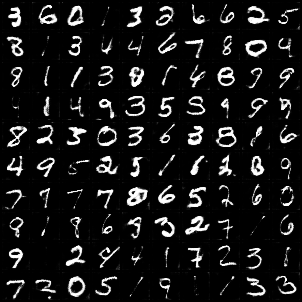
\includegraphics[width=\textwidth]{Img/cg-new.png}
    \caption{CatGAN}
    \label{ffig:m-cg}
  \end{subfigure}
  \begin{subfigure}[b]{\trif\textwidth}
    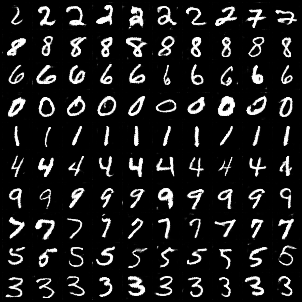
\includegraphics[width=\textwidth]{Img/icg-new.png}
    \caption{InfoCatGAN}
    \label{ffig:m-icg}
  \end{subfigure}
  \begin{subfigure}[b]{\trif\textwidth}
    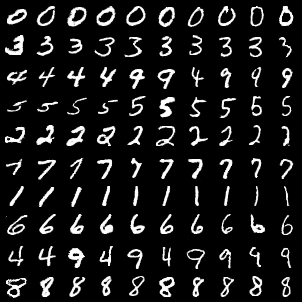
\includegraphics[width=\textwidth]{Img/cig-new.png}
    \caption{C-InfoGAN}
    \label{ffig:m-ig}
  \end{subfigure}

  \begin{subfigure}[b]{\trif\textwidth}
    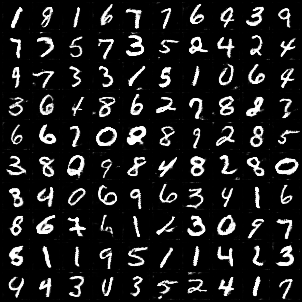
\includegraphics[width=\textwidth]{Img/cg-132labels-new.png}
    \caption{CatGAN(132 labels)}
    \label{ffig:m-ss-cg}
  \end{subfigure}
  \begin{subfigure}[b]{\trif\textwidth}
    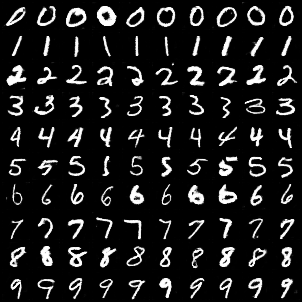
\includegraphics[width=\textwidth]{Img/icg-132labels-new.png}
    \caption{InfoCatGAN(132 labels)}
    \label{ffig:m-ss-icg}
  \end{subfigure}
  \begin{subfigure}[b]{\trif\textwidth}
    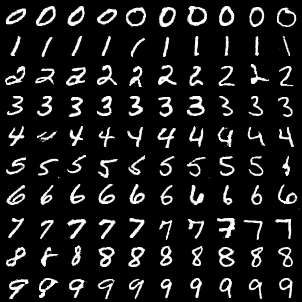
\includegraphics[width=\textwidth]{Img/cig-132labels-new.png}
    \caption{C-InfoGAN(132 labels)}
    \label{ffig:m-ss-ig}
  \end{subfigure}

  \bicaption[模型在MNIST上的生成效果]
  {模型在MNIST上的生成效果。在InfoCatGAN和C-InfoGAN的生成结果中,每一行对应隐变量$c$的一个取值,从0到9。}
  {Generated images on MNIST. Each row corresponds to a value of the categorical latent code $c$, from 0 to 9.}
  \label{fig:mnist}
\end{figure}

图~\ref{ffig:m-ig}和图~\ref{ffig:m-ss-ig}给出了无监督和半监督情况下C-InfoGAN的生成结果。从图中可以看出无监督情况下,模型已经达到了很好的生成效果,隐变量$c$基本可以控制生成图片的类别,但是仍有部分类别未能精确控制(图~\ref{ffig:m-ig});在半监督情况下,隐变量达到了精确的绑定,每一行对应生成一种类别的数字,而且顺序和真实标签是对应的。另外从图~\ref{fig:latent-varies}可以看出,C-InfoGAN模型不仅可以生成指定类别的图片,并且可以通过额外的隐变量调节图片局部特征,如手写数字的粗细,角度等,这对指定特征的数据补足具有很大意义。

\begin{table}[hbtp]
  \renewcommand\arraystretch{0.8} % set row height
  \centering
  \bicaption{模型分类准确率及生成效果}{The accuracy and FID of the Model}
  \label{tab:acc}
  \begin{tabular}{lcccc}
    \toprule
    \multirow{2}{*}{\bf Model} & \multicolumn{2}{c}{\bf MNIST} & \multicolumn{2}{c}{\bf FashionMNIST}\\
    \cline{2-5}
                           & 0 label & 132 labels & 0 label & 100 labels \\ \hline
    ~ & \multicolumn{4}{c}{ACC(\%)} \\ \hline
    CatGAN & \textbf{89.18} & \textbf{98.22} & 67.38 & 71.07  \\
    InfoCatGAN & 87.76 & 96.89 & \textbf{70.61} & 75.24  \\
    C-InfoGAN & 87.59 & 95.85 & 69.57 & \textbf{75.40}   \\
    \hline\hline
    ~ & \multicolumn{4}{c}{FID} \\ \hline
    % DCGAN\cite{radford2015unsupervised} & 113.13 & - & - & - \\
    % VEEGAN\cite{srivastava2017veegan} & 68.75 & - & - & - \\
    % PACGAN\cite{lin2018pacgan} & 58.53 & - & - & - \\
    % PresGAN\cite{dieng2019prescribed} & 42.02 & - & - & - \\
    CatGAN & 37.83 & 21.36 & 69.40 & 67.88  \\
    InfoCatGAN & 12.61 & \textbf{5.99} & 41.17 & 44.36  \\
    C-InfoGAN & \textbf{3.07} & 9.44 & \textbf{11.88} & \textbf{15.99}   \\
    \bottomrule
  \end{tabular}
\end{table}

表~\ref{tab:acc}给出了无监督和半监督情况下模型的分类准确率\footnote{表中有关CatGAN的数据来自与本文复现的结果。},其中ACC表示模型在测试集上的分类准确率,FID表示模型生成图片与真实图片间的FID值,FID越低代表生成质量越好。从表中看出,
InfoCatGAN 的分类准确率虽略低于CatGAN,但在图像生成质量上均一致高于CatGAN,这说明了增加互信息约束可以提高图像的生成质量。在无监督情况下,InfoCatGAN和CatGAN的分类准确率仅相差1.42\%,但FID却比CatGAN降低了25.22,
见图~\ref{ffig:m-icg}。在半监督的情况下,InfoCatGAN的FID达到了5.99。相较于CatGAN模型,C-InfoGAN能够在保证生成质量的同时,达到可观的分类准确率,从表中可以看出,在无监督条件下,C-InfoGAN的生成质量非常好,同时达到了87.59\%的分类准确率。这是因为InfoGAN模型使用的是一个辅助网络$Q$来做类别绑定和分类任务,训练过程中并没有判别器做过多约束,所以无论如何调整分类网络或更改分类约束,也不会对生成效果产生很大影响。这使得模型可以进一步利用生成的图片和标签扩充数据集,以达到更进一步的性能提升。

\begin{table}[htbp]
  \renewcommand\arraystretch{0.7} % set row height
  \centering
  \bicaption{正则系数对InfoCatGAN性能的影响}{The effect of regularization parameter on InfoCatGAN}
  \label{tab:lambda1}
  \begin{tabular}{ccc}
    \toprule
    \textbf{$\lambda_1$} & \textbf{ACC (\%)} & \textbf{FID} \\
    \midrule
    0.0 & 98.22 & 21.36 \\
    0.2 & 97.55 & 18.13 \\
    0.4 & 97.14 & 17.38 \\
    0.9 & 96.89 & 5.99 \\
    \bottomrule
  \end{tabular}
\end{table}
表~\ref{tab:lambda1}给出了正则系数$\lambda_1$(参见\eqref{eq:infocatgan}式)的不同取值对于半监督InfoCatGAN的影响。从表中可以看出,当系数较小时,分类准确率较高,但生成图片的质量较差;当系数较大时,生成的图片效果很好,但分类准确率有所降低。通过调节参数$\lambda_1$,可以实现生成效果和分类准确率之间的折中。实验使用的默认值是$\lambda_1 = 0.9$,当$\lambda_1$减小时,生成图片的质量开始下降,同时分类准确率也会相应增加 ;当$\lambda_1 = 0$时,InfoCatGAN退化为CatGAN。

% 而InfoCatGAN随着正则化系数$\lambda_1$的变化呈现出不同的效果。当系数较小时,分类准确率较高,但生成图片的质量非常差;当系数较大时,生成的图片效果很好,但分类准确率有所降低。实验发现通过调节参数$\lambda_1$,可以实现生成效果和分类准确率之间的折中。实验使用的默认值是$\lambda_1 = 1.1$,
% 当$\lambda_1$减小时,生成图片的质量开始下降,同时分类准确率也会相应增加。值得注意的是,$\lambda_1$越小并不意味着分类准确率越高。当$\lambda_1=0$时,InfoCatGAN退化为CatGAN;而从表~\ref{tab:cat}可以看出,当$\lambda_1=0.02$时,InfoCatGAN的分类准确率高于CatGAN,达到98.15\%。

% \begin{table}[htbp]
%   \centering
%   \bicaption{MNIST分类准确率对比}{Classification accuracy on MNIST}
%   \label{tab:cat}
%   \begin{tabular}{lcc}
%     \toprule
%     \textbf{模型} & \textbf{准确率(\%)} & \textbf{FID} \\
%     \midrule
%     CatGAN & 64.41 & 236.75  \\ 
%     InfoCatGAN & 69.04 & 8.04 \\ 
%     C-InfoGAN & 77.65 & 7.55 \\ 
%     CatGAN(132 labels) & 96.05 & 127.92 \\ 
%     InfoCatGAN(132 labels, $\lambda_1 = 0.02$) & \textbf{98.15} & 169.72 \\
%     InfoCatGAN(132 labels, $\lambda_1 = 0.03$) & 80.43 & \textbf{6.59} \\
%     C-InfoGAN(132 labels) & 93.70 & 9.16 \\
%     \bottomrule
%   \end{tabular}
% \end{table}

%\textcolor{red}{here begins c-infogan} 


\subsection{FashionMNIST}\label{sec:fashion}

FashionMNIST\citep{xiao2017/online}是一个类似MNIST的数据集,二者拥有同样的结构,图像大小,同样的类别数目。但是相对于MNIST,FashionMNIST拥有更复杂的图像结构,以及更难获得非常高的分类准确率,所以对模型更具有检验性。

图~\ref{fig:fashion}中给出了所有模型的生成结果。可以看出,加了互信息约束的模型生成的图片质量均高于CatGAN,并且InfoCatGAN和C-InfoGAN模型均能指定生成图片的类别
,隐变量的每个取值都对应一种类别的图片。
值得一提的是,加入互信息约束后的半监督版本模型从上往下每一行都对应到正确的真实标签。可以看到图~\ref{ffig:ss-icg}和图~\ref{ffig:ss-ig}中对应的顺序一致,这说明隐变量已经正确绑定到真实类别特征。

表~\ref{tab:acc}给出了模型在FashionMNIST的数值结果。
从表中可以看出,在无监督条件下,InfoCatGAN较CatGAN在分类准确率和生成质量上均有所提升,C-InfoGAN在一定程度上兼顾二者,不仅生成质量最优,而且具有相对较高的分类准确率,此外其模型复杂度也较低。在半监督条件下,C-InfoGAN在两个方面均体现出优势,分类准确率达到了75.40\%,FID为15.99,生成效果见图~\ref{ffig:ss-ig}。

\begin{figure}[hbtp]
  \centering
  \begin{subfigure}[b]{\trif\textwidth}
    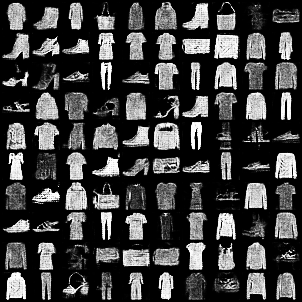
\includegraphics[width=\textwidth]{Img/fa-cg-new.png}
    \caption{CatGAN}
  \end{subfigure}
  \begin{subfigure}[b]{\trif\textwidth}
    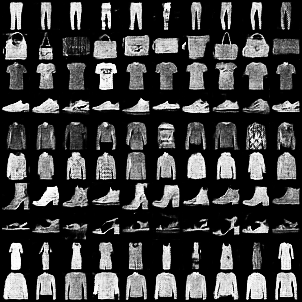
\includegraphics[width=\textwidth]{Img/fa-icg-new.png}
    \caption{InfoCatGAN}
  \end{subfigure}
  \begin{subfigure}[b]{\trif\textwidth}
    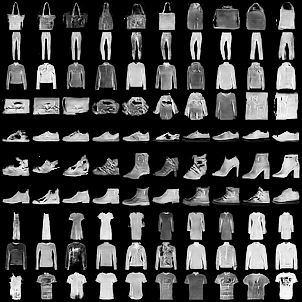
\includegraphics[width=\textwidth]{Img/fa-cig-new.png}
    \caption{C-InfoGAN}
  \end{subfigure}

  \begin{subfigure}[b]{\trif\textwidth}
    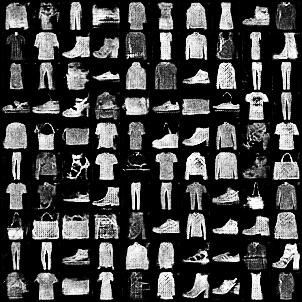
\includegraphics[width=\textwidth]{Img/fa-cg-100labels-new.png}
    \caption{CatGAN(100 labels)}
  \end{subfigure}
  \begin{subfigure}[b]{\trif\textwidth}
    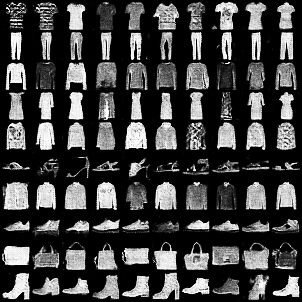
\includegraphics[width=\textwidth]{Img/fa-icg-100labels-new.png}
    \caption{InfoCatGAN(100 labels)}
    \label{ffig:ss-icg}
  \end{subfigure}
  \begin{subfigure}[b]{\trif\textwidth}
    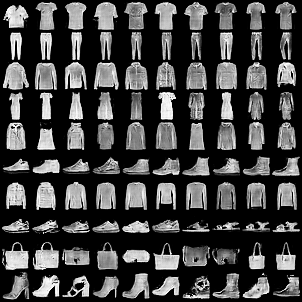
\includegraphics[width=\textwidth]{Img/fa-cig-100labels-new.png}
    \caption{C-InfoGAN(100 labels)}
    \label{ffig:ss-ig}
  \end{subfigure}

  \bicaption[模型在FashionMNIST上的生成效果]
  {模型在FashionMNIST上的生成效果。在InfoCatGAN和C-InfoGAN的生成结果中,每一行对应隐变量$c$的一个取值,从0到9。}
  {Generated images on FashionMNIST. Each row corresponds to a value of the categorical latent code $c$, from 0 to 9.}
  \label{fig:fashion}
\end{figure}
% 从表中可以看出,无论是在无监督还是半监督情况下,C-InfoGAN的分类准确率都是比较高的。在无监督情况下,InfoCatGAN提高了生成图片的质量,但与此同时,牺牲了分类准确率,而C-InfoGAN在一定程度上二者兼顾,不仅生成质量最优,而且具有相对较高的分类准确率,此外其模型复杂度也较低。在半监督情况下,InfoCatGAN在两个方面均体现出优势,分类准确率达到了74.21\%,FID为$16.92$,生成效果见图~\ref{ffig:ss-icg},这说明增加标签信息对模型的增益很大。
% \begin{table}[htbp]
%   \centering
%   \bicaption{FashionMNIST分类准确率对比}{Classification accuracy on FashionMNIST}
%   \label{tab:fashion}
%   \begin{tabular}{lcc}
%     \toprule
%     \textbf{模型} & \textbf{准确率(\%)} & \textbf{FID} \\
%     \midrule
%     CatGAN & 64.28 & 120.04  \\ 
%     InfoCatGAN & 57.66 & 26.43 \\ 
%     C-InfoGAN & 60.50 & 15.97 \\ 
%     CatGAN(100 labels) & 73.34 & 119.16 \\ 
%     InfoCatGAN(100 labels) & \textbf{74.21} & 16.92 \\ 
%     C-InfoGAN(100 labels) & 68.94 & \textbf{15.94} \\
%     \bottomrule
%   \end{tabular}
% \end{table}

\subsection{可解释性}
从以上结果可以看出,加入互信息约束可以给模型带来许多增益,其中最为显著的是生成质量的提升。图~\ref{fig:phase}给出了MNIST数据集下InfoCatGAN在训练的不同阶段对应的生成效果。其中,$L_I$是公式\eqref{eq:vlb}中的互信息下界,可以看到,随着隐变量$c$和生成数据$\tilde{x}$的互信息增加,生成的图片开始具有绑定效果,并且生成的图像越来越好。

\begin{figure}[htbp]
  \centering
  \begin{subfigure}[b]{\trif\textwidth}
    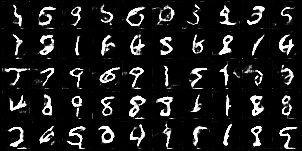
\includegraphics[width=\textwidth]{Img/fake-epoch-5.png}
    \caption{Epoch 5, $L_I=0.0338$}
  \end{subfigure}
  \begin{subfigure}[b]{\trif\textwidth}
    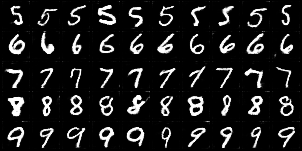
\includegraphics[width=\textwidth]{Img/fake-epoch-100.png}
    \caption{Epoch 100, $L_I=0.5809$}
  \end{subfigure}
  \begin{subfigure}[b]{\trif\textwidth}
    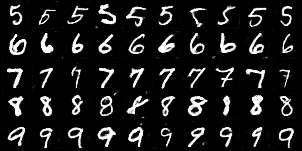
\includegraphics[width=\textwidth]{Img/fake-epoch-300.png}
    \caption{Epoch 300, $L_I=1.5332$}
  \end{subfigure}

  \bicaption{InfoCatGAN不同阶段的生成效果}{Generated samples of InfoCatGAN at different phases}
  \label{fig:phase}
\end{figure}

对于InfoCatGAN在生成质量上的增益,本文参考\citet{spurr2017guiding}从互信息的角度给出一些直观解释。由公式\eqref{eq:lcatg}、 \eqref{eq:infocatgan}可知,生成器$G$的优化目标是最大化$I(\tilde{X}; Y)$和$I(\tilde{X};C)$,这可以令虚假标签$c$和真实标签$y$对应;而半监督条件下判别器$D$的目标是最大化$I(X;Y)$,以及最小化真实分布和预测分布之间的交叉熵$\E_{p(y|x)}\log\frac{1}{p(c|x)}$,进而使得真实标签$y$中的信息流入隐变量$c$,此处$X,~\tilde{X},~Y,~C$分别代表真实数据、生成数据、真实标签、虚假标签所对应的随机变量。事实上在半监督版本的InfoCatGAN中,本文就是采用$c$的后验概率$p(c|\cdot) = D(\cdot)$作为模型的预测值,从实验结果也可以看出虚假标签和真实标签是正确对应的(图~\ref{ffig:m-ss-icg})。换句话说,模型的优化目标变为$I(C;X)$和$I(C;\tilde{X})$。现假设:
\begin{enumerate}
  \item $X \leftarrow C \rightarrow \tilde{X}$:箭头表示依赖关系,这个假设来 源于图像是由多个独立隐变量的相互作用生成的,实际中这些隐变量还包括噪声$Z$,以及其他因素。为了简单起见,这里假设只和隐变量$C$有关。
  \item 初始时$I(X;\tilde{X})=0$:开始的时候,虚假数据和真实数据无关。
  \item $H(C)$为定值:假设$C$的先验分布在训练过程中没有改变,所以它的熵是确定的。
\end{enumerate}
由\citet{spurr2017guiding},$H(C)$可分解为:
\[
  H(C) = I(C;X) + I(C;\tilde{X}) + H(C|X,\tilde{X}) - I(X;\tilde{X}) + I(X;\tilde{X}|C).
\]
由假设1,
\[
  H(C) = I(C;X) + I(C;\tilde{X}) + H(C|X,\tilde{X}) - I(X;\tilde{X}).
\]
由假设3,
\[
  0 = \Delta I(C;X) + \Delta I(C;\tilde{X}) + \Delta H(C|X,\tilde{X}) - \Delta I(X;\tilde{X}),
\]
其中$\Delta$表示变化量。进一步得到以下两种情况:
\begin{align}
  \Delta I(C;X) + \Delta I(C;\tilde{X}) &\ge -\Delta H(C|X,\tilde{X}) \implies \Delta I(X;\tilde{X}) \ge 0, \label{case1} \\
  \Delta I(C;X) + \Delta I(C;\tilde{X}) &\le -\Delta H(C|X,\tilde{X}) \implies \Delta I(X;\tilde{X}) \le 0. \label{case2}
\end{align}
注意到模型的训练目标是最大化两个互信息,所以上式左边一定为正值。由假设2,初始时$I(X;\tilde{X})=0$,如果第二种情况发生,则会导致$I(X;\tilde{X})$变为负值,而互信息是非负的,因此第二种情况不会发生。于是得到,同时增加$I(C;X)$和$I(C;\tilde{X})$会导致$I(X;\tilde{X})$增加,这也就说明了生成图片与真实图片更为接近,即模型的生成质量较好。

\begin{figure}[htbp]
  \centering
  \begin{subfigure}[b]{\twof\textwidth}
    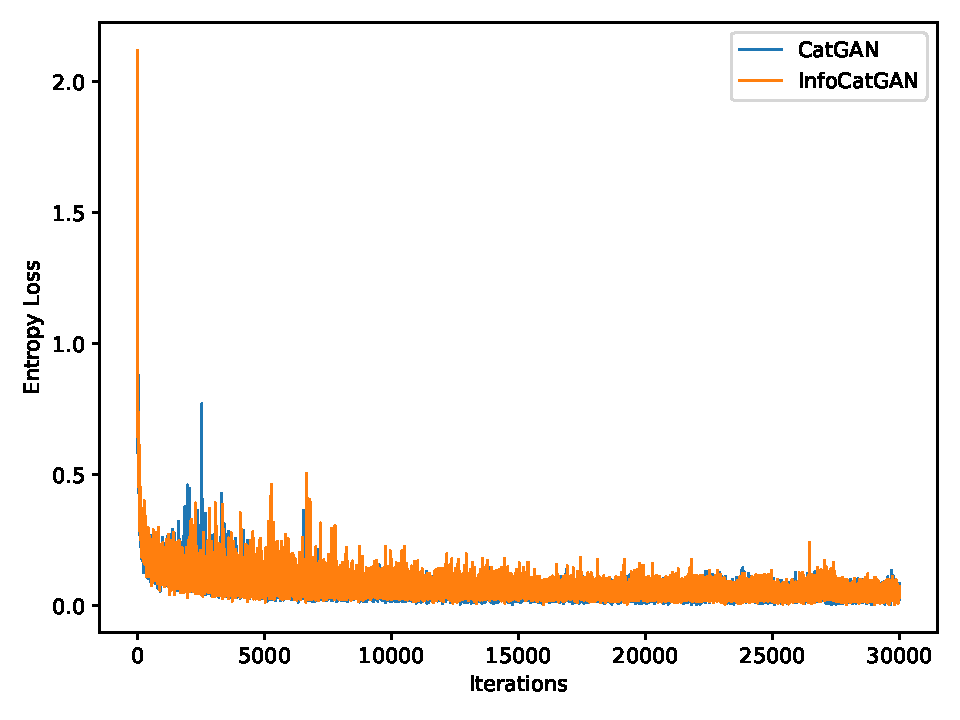
\includegraphics[width=\textwidth]{Img/icg-convergence.pdf}
    \caption{Entropy loss of CatGAN and InfoCatGAN}
    \label{ffig:icg-convergence}
  \end{subfigure}
  \begin{subfigure}[b]{\twof\textwidth}
    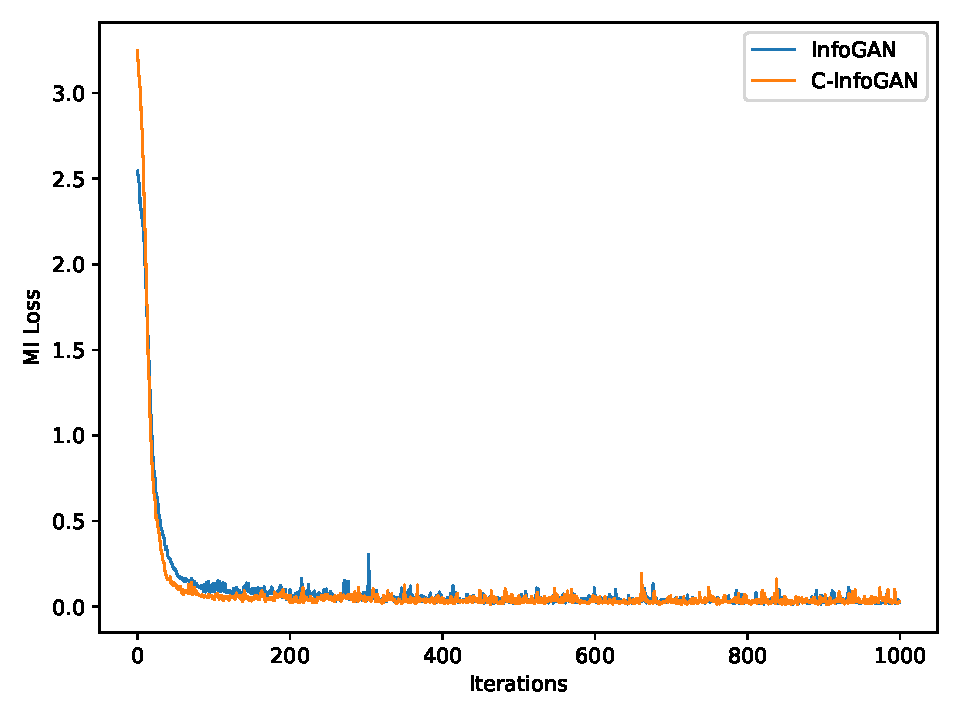
\includegraphics[width=\textwidth]{Img/cig-convergence.pdf}
    \caption{MI loss of InfoGAN and C-InfoGAN}
    \label{ffig:cig-convergence}
  \end{subfigure}
  \bicaption{模型在MNIST上的收敛速度}{Convergence speed on MNIST}
  \label{fig:convergence}
\end{figure}
\subsection{收敛速度分析}
本文提出的两个模型在原理上都属于正则化生成对抗网络,因此相较于原先的两个模型CatGAN和InfoGAN,增加的计算复杂度很小。由于GAN的训练方式特殊,训练的过程是两个模块间的对抗,因此目前没有一个统一的评判收敛性的标准。针对InfoCatGAN和C-InfoGAN两种模型,本文分别用条件熵损失(即判别器输出的概率分布对应的熵)以及互信息损失(实际采用交叉熵估计,详见\ref{sec:c-infogan}节)来作为模型收敛的佐证,见图~\ref{fig:convergence}。

\section{本章小结}
本章分别给出了InfoCatGAN和C-InfoGAN在两个数据集MNIST和FashionMNIST上的实验结果。从结果来看,InfoCatGAN相比于CatGAN牺牲了一点分类准确率,但在图片生成质量上有很大的提升。此外,该模型可以通过调节正则化系数达到生成质量和分类准确率之间的折中。C-InfoGAN具有良好的生成质量和可观的分类准确率,并且可以通过隐变量控制图片的局部细节。值得注意的是,两个模型均能利用隐变量的取值来控制生成图片的类别,这对数据增强具有较大的意义。
